114. \begin{figure}[ht!]
\center{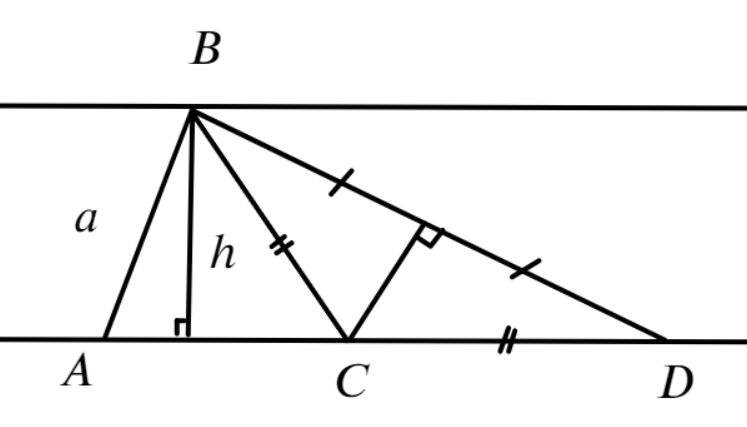
\includegraphics[scale=0.35]{g114.png}}
\end{figure}\\
Сначала построим две параллельные прямые, расстояние между которыми равно высоте $h.$ Затем выберем на одной из них точку $A$ и проведём окружность радиуса $a,$ пусть она пересечёт вторую прямую в точке $B$ (если не пересечёт, то искомого треугольника не существует). Отложим от точки $A$ отрезок $AD=b+c.$ Построим серединный перпендикуляр к отрезку $BD,$ пусть он пересечёт $AD$ в точке $C.$ Так как $BC=CD,\ AC+BC=AC+CD=b+c,$ значит треугольник $ABC$ --- искомый.\newpage\noindent
